%%%%%%%%%%%%%%%%%%%%%%%%%%%%%%%%%%%%%%%%%%%%%%%%%%%%%%%%%%%%%%%%%%%%%%%%%%%%%%%%%%%%%%%%%%%%%%%%%
%
% Document:     Data Management  product tree
%
%%%%%%%%%%%%%%%%%%%%%%%%%%%%%%%%%%%%%%%%%%%%%%%%%%%%%%%%%%%%%%%%%%%%%%%%%%%%%%
\documentclass{article}
\usepackage{times,layouts}
\usepackage{tikz,hyperref,amsmath}
\usetikzlibrary{positioning,arrows,shapes,decorations.shapes,shapes.arrows}
\usetikzlibrary{backgrounds,calc}
\usepackage[paperwidth=36.4cm,paperheight=14.540000000000001cm,
left=-2mm,top=3mm,bottom=0mm,right=0mm,
noheadfoot,marginparwidth=0pt,includemp=false,
textwidth=30cm,textheight=50mm]{geometry}
\newcommand\showpage{%
\setlayoutscale{0.5}\setlabelfont{\tiny}\printheadingsfalse\printparametersfalse
\currentpage\pagedesign}
\hypersetup{pdftitle={DM products }, pdfsubject={Diagram illustrating the
                products in LSST DM }, pdfauthor={Autogenerated from MD}}
\tikzstyle{tbox}=[rectangle,text centered, text width=30mm]
\tikzstyle{wbbox}=[rectangle, rounded corners=3pt, draw=black, top color=blue!50!white,
                    bottom color=white, very thick, minimum height=12mm, inner sep=2pt,
                    text centered, text width=30mm]
\tikzstyle{pbox}=[rectangle, rounded corners=3pt, draw=black, top
 color=yellow!50!white, bottom color=white, very thick,
 minimum height=35pt, inner sep=2pt, text centered, text width=35mm]
\tikzstyle{pline}=[-, thick]
\begin{document}
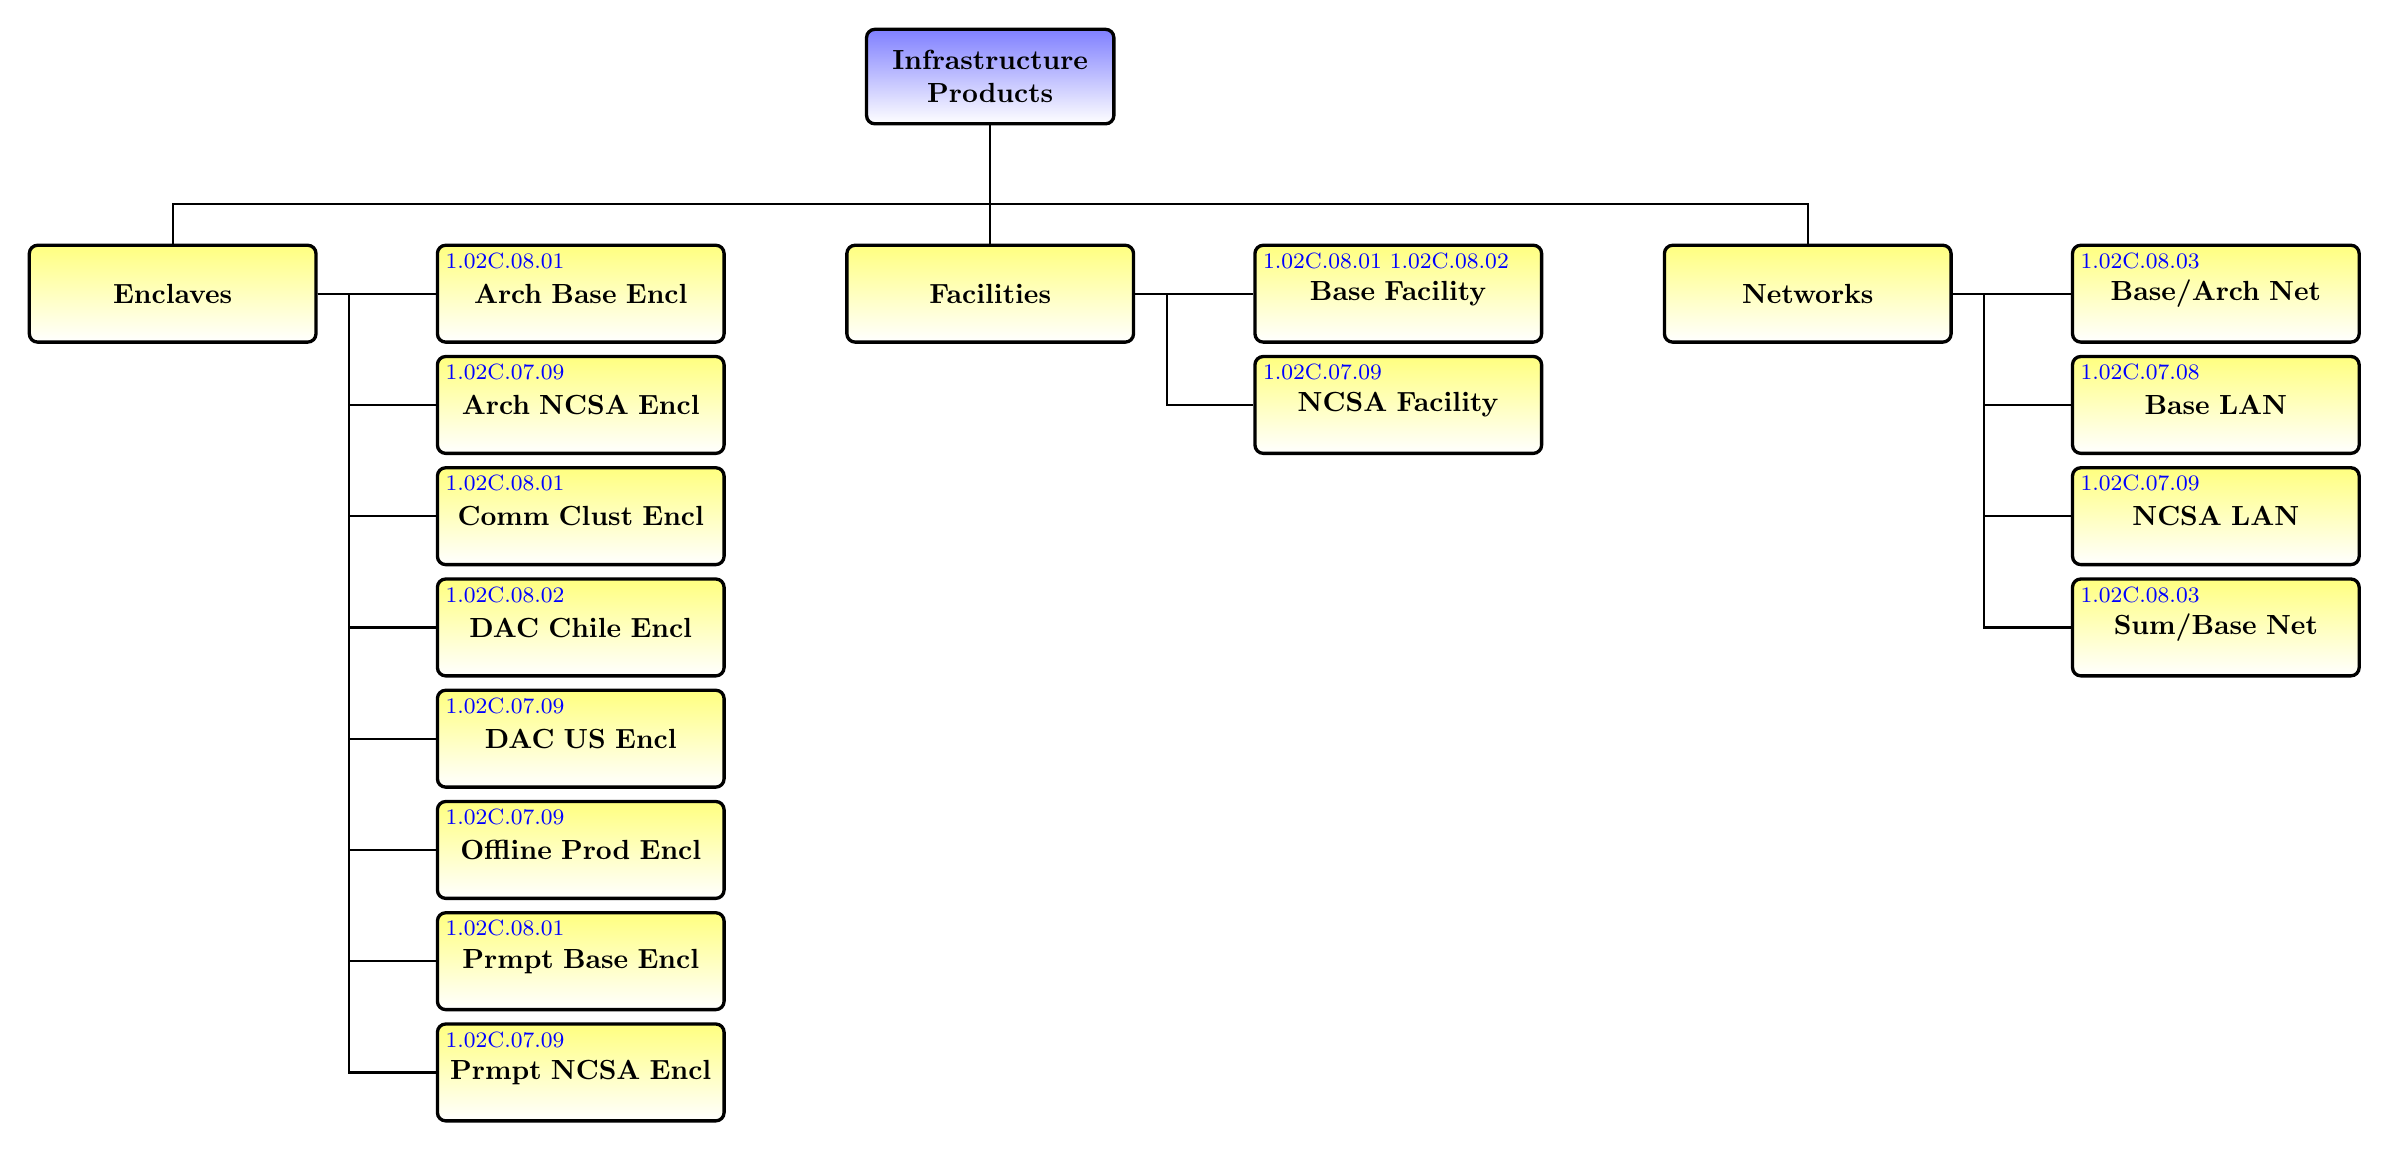
\begin{tikzpicture}[node distance=0mm]


\node (ENC) [pbox, 
] {\textbf{Enclaves
} };
\node [below right] at (ENC.north west) {\footnotesize \color{blue}} ;
\node (ENCARCB) [pbox,right=15mm of ENC] {\textbf{Arch Base Encl
} };
\node [below right] at (ENCARCB.north west) {\footnotesize \color{blue}1.02C.08.01} ;
 \draw[pline] (ENC.east) -| ++(0.4,0) |- (ENCARCB.west); 
\node (ENCARCN) [pbox,below=4pt of ENCARCB] {\textbf{Arch NCSA Encl
} };
\node [below right] at (ENCARCN.north west) {\footnotesize \color{blue}1.02C.07.09} ;
 \draw[pline] (ENC.east) -| ++(0.4,0) |- (ENCARCN.west); 
\node (ENCCOMM) [pbox,below=4pt of ENCARCN] {\textbf{Comm Clust Encl
} };
\node [below right] at (ENCCOMM.north west) {\footnotesize \color{blue}1.02C.08.01} ;
 \draw[pline] (ENC.east) -| ++(0.4,0) |- (ENCCOMM.west); 
\node (ENCDACC) [pbox,below=4pt of ENCCOMM] {\textbf{DAC Chile Encl
} };
\node [below right] at (ENCDACC.north west) {\footnotesize \color{blue}1.02C.08.02} ;
 \draw[pline] (ENC.east) -| ++(0.4,0) |- (ENCDACC.west); 
\node (ENCDACU) [pbox,below=4pt of ENCDACC] {\textbf{DAC US Encl
} };
\node [below right] at (ENCDACU.north west) {\footnotesize \color{blue}1.02C.07.09} ;
 \draw[pline] (ENC.east) -| ++(0.4,0) |- (ENCDACU.west); 
\node (ENCOFFL) [pbox,below=4pt of ENCDACU] {\textbf{Offline Prod Encl
} };
\node [below right] at (ENCOFFL.north west) {\footnotesize \color{blue}1.02C.07.09} ;
 \draw[pline] (ENC.east) -| ++(0.4,0) |- (ENCOFFL.west); 
\node (ENCPRB) [pbox,below=4pt of ENCOFFL] {\textbf{Prmpt Base Encl
} };
\node [below right] at (ENCPRB.north west) {\footnotesize \color{blue}1.02C.08.01} ;
 \draw[pline] (ENC.east) -| ++(0.4,0) |- (ENCPRB.west); 
\node (ENCPRN) [pbox,below=4pt of ENCPRB] {\textbf{Prmpt NCSA Encl
} };
\node [below right] at (ENCPRN.north west) {\footnotesize \color{blue}1.02C.07.09} ;
 \draw[pline] (ENC.east) -| ++(0.4,0) |- (ENCPRN.west); 
\node (FAC) [pbox, 
right=6.7cm of ENC] {\textbf{Facilities
} };
\node [below right] at (FAC.north west) {\footnotesize \color{blue}} ;
\node (FACBASE) [pbox,right=15mm of FAC] {\textbf{Base Facility
} };
\node [below right] at (FACBASE.north west) {\footnotesize \color{blue}1.02C.08.01 1.02C.08.02} ;
 \draw[pline] (FAC.east) -| ++(0.4,0) |- (FACBASE.west); 
\node (FACNCSA) [pbox,below=4pt of FACBASE] {\textbf{NCSA Facility
} };
\node [below right] at (FACNCSA.north west) {\footnotesize \color{blue}1.02C.07.09} ;
 \draw[pline] (FAC.east) -| ++(0.4,0) |- (FACNCSA.west); 
\node (NET) [pbox, 
right=6.7cm of FAC] {\textbf{Networks
} };
\node [below right] at (NET.north west) {\footnotesize \color{blue}} ;
\node (NETBA) [pbox,right=15mm of NET] {\textbf{Base/Arch Net
} };
\node [below right] at (NETBA.north west) {\footnotesize \color{blue}1.02C.08.03} ;
 \draw[pline] (NET.east) -| ++(0.4,0) |- (NETBA.west); 
\node (NETBASE) [pbox,below=4pt of NETBA] {\textbf{Base LAN
} };
\node [below right] at (NETBASE.north west) {\footnotesize \color{blue}1.02C.07.08} ;
 \draw[pline] (NET.east) -| ++(0.4,0) |- (NETBASE.west); 
\node (NETNCSA) [pbox,below=4pt of NETBASE] {\textbf{NCSA LAN
} };
\node [below right] at (NETNCSA.north west) {\footnotesize \color{blue}1.02C.07.09} ;
 \draw[pline] (NET.east) -| ++(0.4,0) |- (NETNCSA.west); 
\node (NETSB) [pbox,below=4pt of NETNCSA] {\textbf{Sum/Base Net
} };
\node [below right] at (NETSB.north west) {\footnotesize \color{blue}1.02C.08.03} ;
 \draw[pline] (NET.east) -| ++(0.4,0) |- (NETSB.west); 
\node (INFRA) [wbbox, above=15mm of FAC]{\textbf{Infrastructure Products}};
 \draw[pline]   (ENC.north) -- ++(0.0,0.5) -| (INFRA.south) ; 
 \draw[pline]   (FAC.north) -- ++(0.0,0.5) -| (INFRA.south) ; 
 \draw[pline]   (NET.north) -- ++(0.0,0.5) -| (INFRA.south) ; 

\end{tikzpicture}
\end{document}
